\subsection{SonelGaz:}

Sonelgaz est l'opérateur historique dans le domaine de la fourniture des énergies électrique et gazière en Algérie. Crée en 1969, Sonelgaz, œuvre depuis un demi-siècle au service du citoyen algérien en lui apportant cette source énergétique essentielle à la vie quotidienne.

\begin{figure}[h]
	\centering
    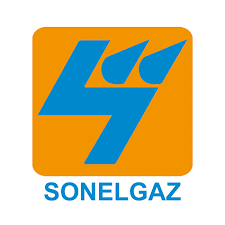
\includegraphics[scale=1]{img/part2/1.6}
    \caption{Logo SonelGaz}
\end{figure}

A la faveur de la promulgation de la loi sur l'électricité et la distribution du gaz par canalisations, Sonelgaz est passée d'une entreprise verticalement intégrée à une holding pilotant un Groupe industriel multi-sociétés et multi-métiers.

Sonelgaz a toujours joué un rôle majeur dans le développement économique et social du pays. Sa contribution dans la concrétisation de la politique énergétique nationale est à la mesure des importants programmes réalisés, en matière d'électrification rurale et de distribution publique gaz ; ce qui a permis de hisser le taux de couverture en électricité à 98\% pour 10 494 000 clients et un taux de pénétration du gaz à 65\% pour 6 451 000 clients. Aujourd’hui, le groupe Sonelgaz est composé de 21 sociétés dont 02 Holding, dont 14 sociétés directement pilotées par la Holding, 02 sociétés contrôlées à hauteur de 50 et 51\% et de 05 sociétés en participations avec des tiers.